\documentclass{subfile}

\begin{document}
  \section{Appendix}
  Key figures used for observations or minature version used will be provided in larger scale.
  \begin{figure}[!h]
  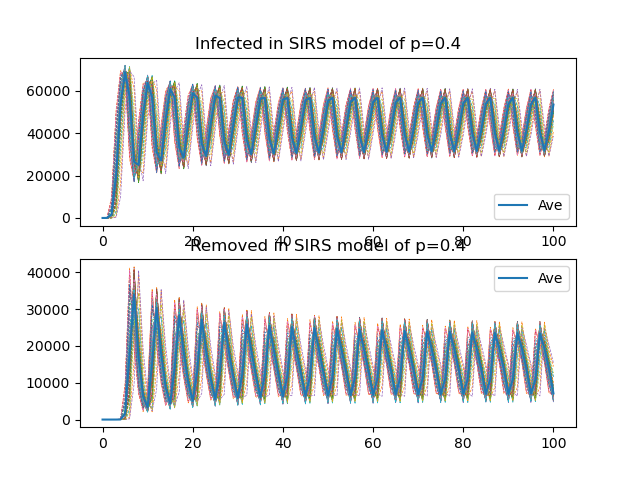
\includegraphics[scale=0.8]{sirsp04r1i3s3}
  \caption[SIRS p=0.4,r=1,i=3,init infected=3]{SIRS Model with p=0.4 r=1 i=3 initial infected=3 simulation using Snap.py}
  \end{figure}
  \begin{figure}
  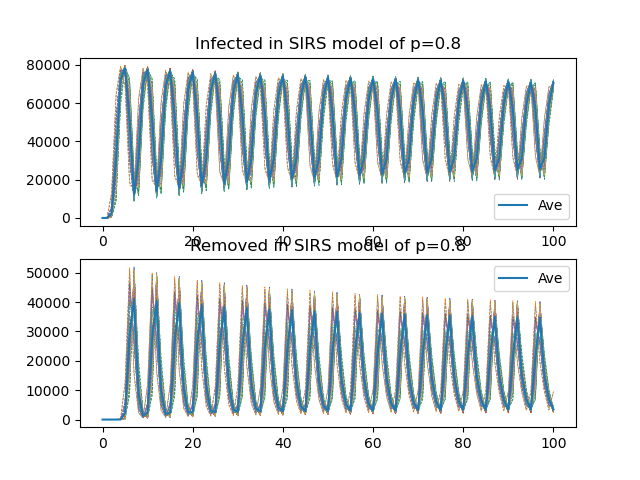
\includegraphics[scale=0.8]{sirsp08r1i3s3}
  \caption[SIRS p=0.8,r=1,i=3,init infected=3]{SIRS Model with p=0.8 r=1 i=3 initial infected=3 simulation using Snap.py}
  \end{figure}
  \begin{figure}
  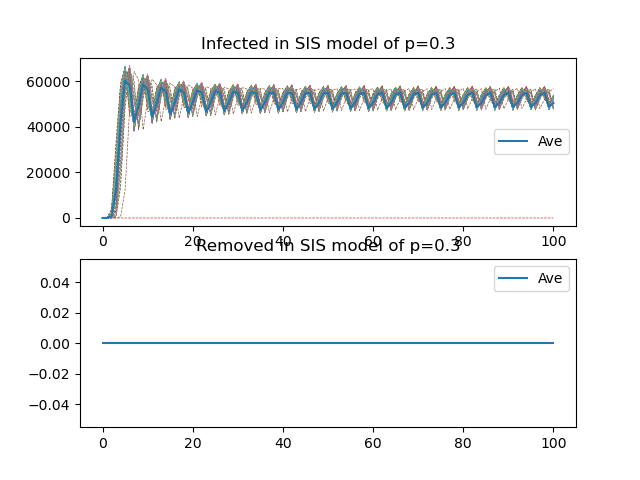
\includegraphics[scale=0.8]{sisp03r1i3s3}
  \caption[SIS p=0.3,r=1,i=3,init infected=3]{SIS Model with p=0.3 r=1 i=3 initial infected=3 simulation using Snap.py}
  \end{figure}
  \begin{figure}
  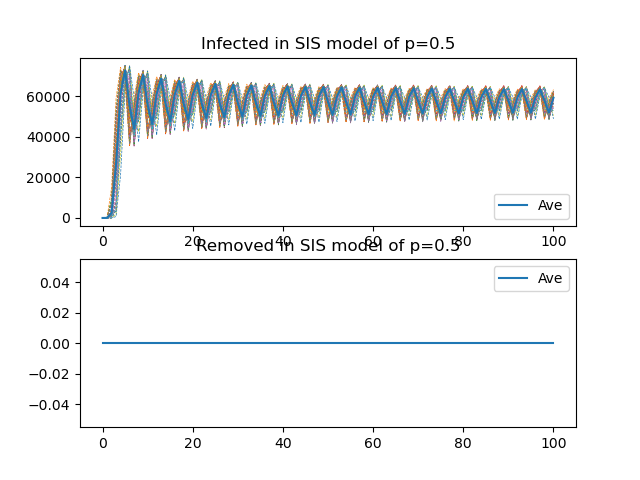
\includegraphics[scale=0.8]{sisp05r1i3s3}
  \caption[SIS p=0.5,r=1,i=3,init infected=3]{SIS Model with p=0.5 r=1 i=3 initial infected=3 simulation using Snap.py}
  \end{figure}
  \begin{figure}
  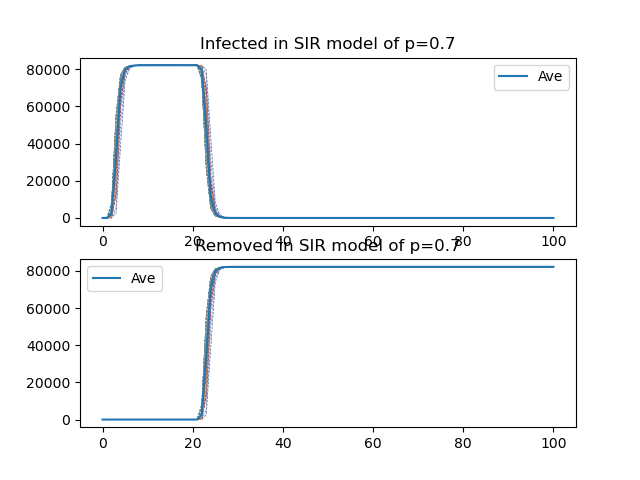
\includegraphics[scale=0.8]{sirp07r1i20s3}
  \caption[SIR p=0.7,r=1,i=20,init infected=3]{SIR Model with p=0.7 r=1 i=20 initial infected=3 simulation using Snap.py}
  \end{figure}
  \begin{figure}
  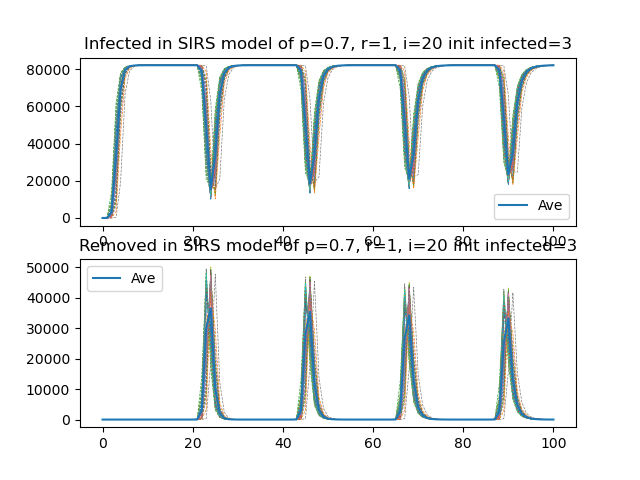
\includegraphics[scale=0.8]{sirsp07r1i20s3}
  \caption[SIRS p=0.7,r=1,i=20,init infected=3]{SIRS Model with p=0.7 r=1 i=20 initial infected=3 simulation using Snap.py}
  \end{figure}
  \begin{figure}
  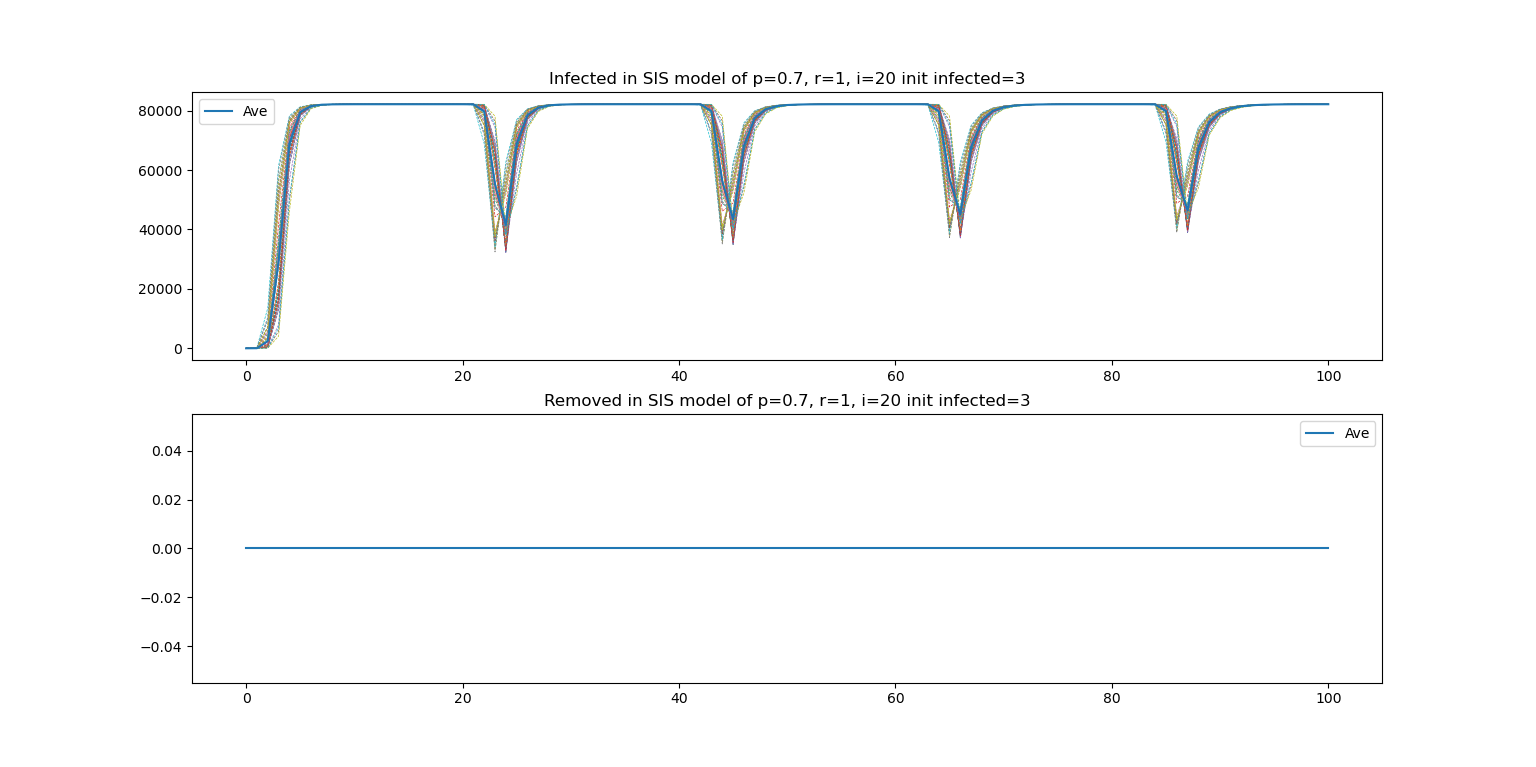
\includegraphics[scale=0.8]{sisp07r1i20s3}
  \caption[SIS p=0.7,r=1,i=20,init infected=3]{SIS Model with p=0.7 r=1 i=20 initial infected=3 simulation using Snap.py}
  \end{figure}

  \clearpage
\end{document}
